\documentclass[10pt,a4paper]{article}
\usepackage{listings}
\usepackage[utf8]{inputenc}
\usepackage{color}
\usepackage[francais]{babel}
\usepackage[T1]{fontenc}
\usepackage{graphicx}
\usepackage[export]{adjustbox}
\bibliographystyle{ieeetr}
\author{Ali CHERIFI, Clément FONTENAY, Valentin GAILLARD}
\title{Projet de compilation\\Intepréteur de Pseudo-Pascal \\Traducteur de Pseudo-Pascal vers C3A}

\begin{document}
\maketitle
\newpage
\tableofcontents
\newpage
\section{Introduction}

Le but de ce projet est de manipuler la théorie des langages via les outils Bison et Flex sur le langage Pseudo-Pascal.
Ce langage est assez complet puisqu'il gère le typage des variables (booléen et entier), les tableaux, les appels de fonctions ainsi que la portée des variables.
Nous avons pour cela à réaliser les programmes suivant :\\ 
\begin{itemize}
    \item Un interpréteur de Pseudo-Pascal.
    \item Un traducteur de Pseudo-Pascal vers C3A (code à 3 adresses).
    \item Un interpréteur de C3A.
\end{itemize}

\section{Cahier des charges}
\subsection{Besoins fonctionnels}

\begin{itemize}
    \item Prendre en entrée un programme Pseudo-Pascal au format .pp.
    \item Vérifier que le programme est correct syntaxiquement et sémantiquement.
    \item Interpréter ce programme pour en dégager le résultat.
    \item Traduire le programme en C3A.
    \item Interpréter ce programme C3A.
\end{itemize}

\subsection{Besoins non foncitonnels}

\begin{itemize}
    \item Indication sur les erreurs commises par l'utilisateur lors de l'écriture du programme Pseudo-Pascal.
    \item Traduction du programme relativement rapide.\\
\end{itemize}

Nous ne traiterons pas les options demandées c'est-à-dire le passage au langage assembleur Y86 et le ramasse-miettes.
Nous avons fait le choix de nous concentrer sur les fonctionnalités principales afin de les implémenter de la meilleure manière possible.

\subsection{Architecture}
Nous avons découpés notre travail de façon à créer plusieurs modules qui peuvent être assemblés par la suite.


\begin{itemize}
    \item Les fichiers .y et .l permettent la lecture du programme d'entrée et l'analyse syntaxique.
    \item Le module d'analyse sémantique se trouve dans les fichiers analyseur.c/.h
    \item L'interpréteur se trouve dans le fichier interpreteur.c
\end{itemize}

Notre arbre, où est stocké le code du corps, \textit{C} dans la grammaire,  est constitué de structure \textit{NOE}. Les fonctions sont stockées dans une structure \textit{BILFON}, contenant leurs noms, leurs paramètres, leurs variables locales ainsi que leurs corps. Et enfin, les variables globales sont stockées dans une structure \textit{BILENV}. Ces trois stuctures sont ensuite stockés dans une structure \textit{EnvGloabal}; qui est utilisés dans les différentes fonctions d'interprétation et de traduction.
  
\begin{figure}
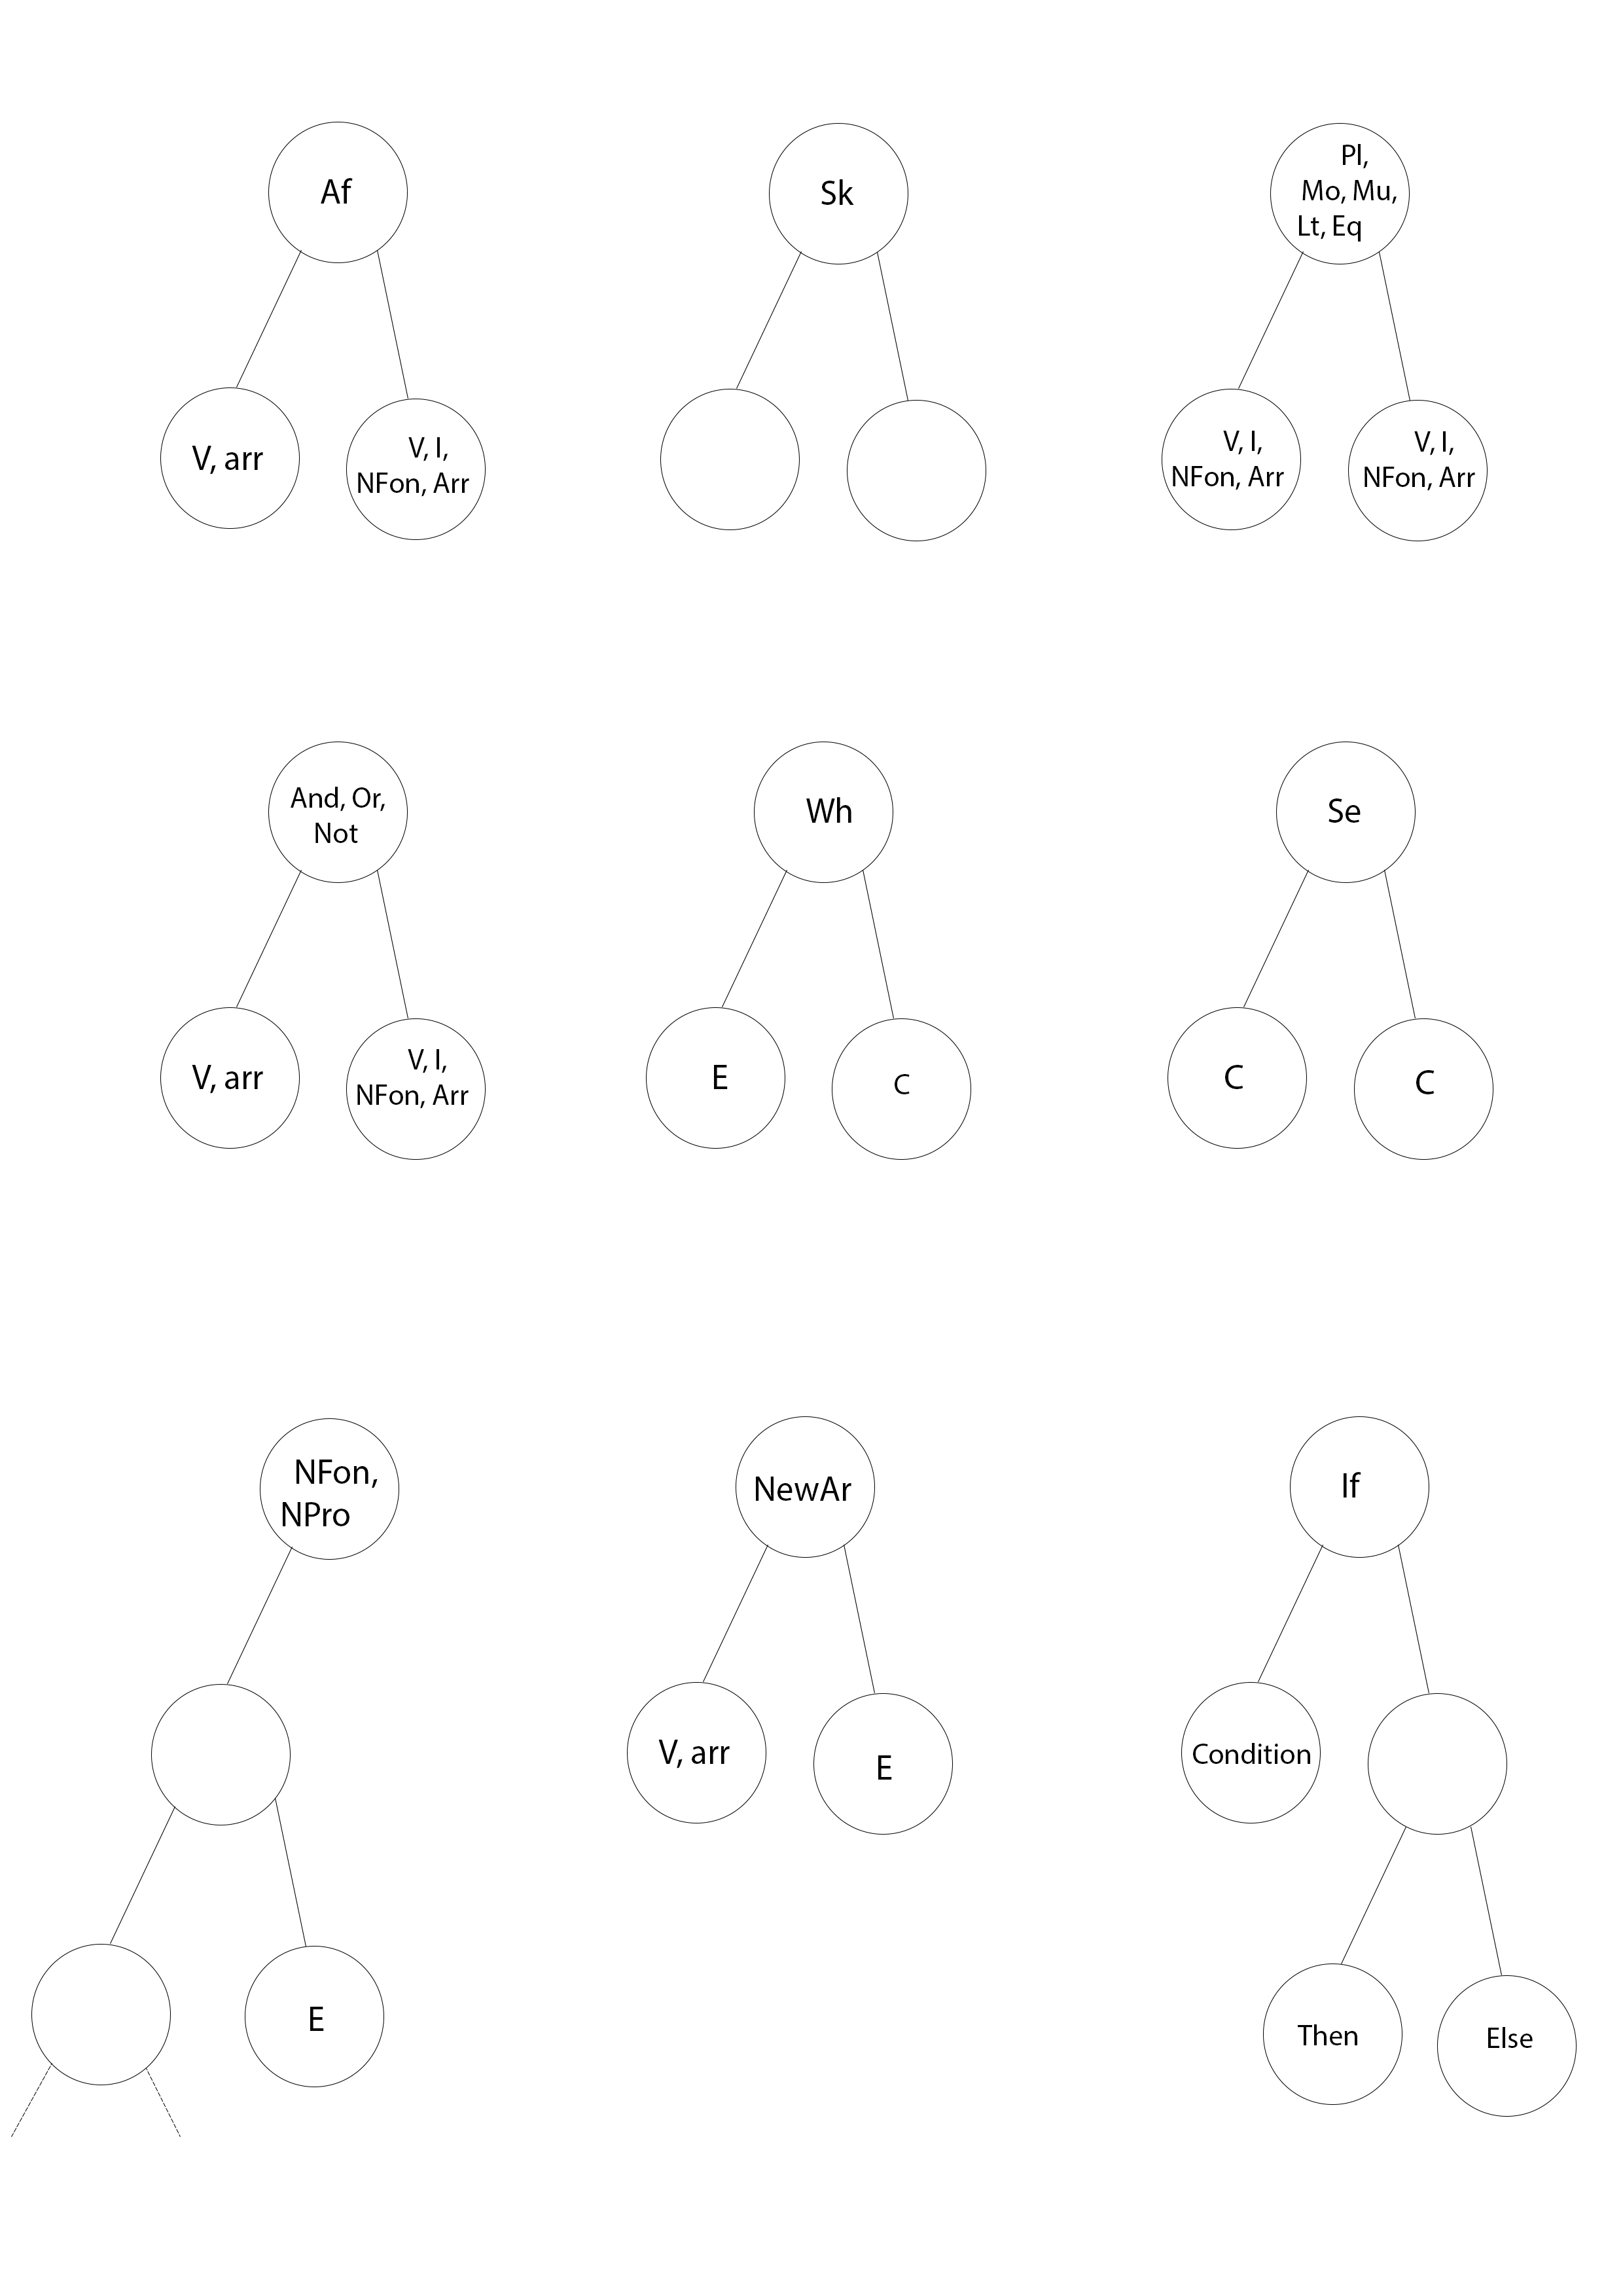
\includegraphics[scale = 0.17]{compi.png}
\caption{\textit{Les noeuds utilisés}.}
\label{SchemaNoeuds}
\end{figure}
\newpage

\section{Implémentation}
\subsection{Description globale}
Pour analyser et par la suite interpréter notre programme nous nous sommes reposé sur la lecture faite par Bison.
Bison pouvant générer un arbre du programme lu via sa grammaire, nous pouvons par la suite lire cet arbre par un parcours préfixe et donc l'interpréter.

Nous avons implémenté une structure de noeud comportant les champs codop (Code de l'opération en cours), \textit{ETIQ} (Nom de variable, valeur, etc..), \textit{FG}, \textit{FD} 
(respectivement fils gauche et fils droit). Dans notre grammaire les commandes et expressions sont de type noeud ce qui nous permet de construire l'arbre du programme.

Nous disposons également de notre propre structure \textit{EnvG} qui regroupe la totalité du programme lu via un \textit{BILENV} stockant les variables globales, un noeud 
racine comportant tout le programme principal (sans les déclarations de fonctions auxiliaires) et une liste \textit{BILFON} répertoriant les déclarations de fonctions. 
Le non-terminal MP est de type \textit{EnvG}, l'interpréteur (ou le traducteur) à alors accès à tous les éléments composant un programme.

\subsection{Description de l'analyseur sémantique}
Tout d'abord pour chaque utilisation d'une variable, nous regardons si elle est définie. Pour ça, nous recherchons dans \textit{ListeVariablesLOCALES} puis dans \textit{ListeVariablesGLOBALES}. Nous remplissons \textit{ListeVariablesLocales} à chaque fois fois qu'il y a une définition de fonction pour y mettre dedans les paramètres de la fonction; puis nous rajoutons à la liste , les variables déclarées dans la fonction, en vérifiant qu'il n'y est pas ddeux variables portant le même nom.
Après cette vérification, nous vérifions que les types sont cohérents, pour les affectations, les appels de fonctions, les opérations ...Et nous finissons par afficher le message adéquat et la ligne.


L'analyseur sémantique vérifie donc:\newline
\begin{itemize}
    \item Les variables déclarées dans le même bloc, ne peuvent avoir le même nom
    \item Les fonctions ne peuvent avoir le même nom
    \item Les procédures ne peuvent renvoyer de valeur
    \item Les opérations logiques ne peuvent être utlisées seulement avec des types booléen
    \item Les opérations arithmétique ne peuvent être utilisées seulement avec des types entier
    \item Les affectations doivent avoir le même type à gauche et à droite
    \item A l'appel d'une fonction, les paramètres envoyés doivent être du bon type et leurs nombres aussi
\end{itemize}


\subsection{Description du traducteur C3A}
Sachant que le code a été vérifié par les analyseurs, nous parcourons récursivement l'arbre construit par le bison. Nous traduisons donc ligne par ligne en incrémentant un compteur global pour les étiquettes. Comme nous n'avons pas d'instructions pour les déclarations des variables locales, nous renommons celles qui ont le même noms que les globales, dans les instructions \textit{param} ainsi que dans le corps des fonctions. Nous rajoutons la tradution des fonctions à la fin du fichier traduit, chaque fonction commence à l'étiquette portant son nom.
\subsection{Problèmes rencontrés et solutions}
\subsubsection{Pour l'analyseur lexical}
Le premier problème était de récupérer le nom des variables, donc pour ça nous avons d'abord essayer en rajoutant simplement, dans l'union yylval, un char* nom, mais n'étant pas la bonne solution puisqu'en construisant l'arbre avec bison, yylval.nom n'avait pas la bonne valeur au bon moment. Donc pour solutionner ce problème nous avons rendu V terminal, pour ça nous avons rajouté yylval.noeud; et c'est dans le flex, au moment de lire une variable, que nous créons un nouveau noeud et que nous mettons dans yylval.noeud.

Le second problème, qui était sans doute le plus petit, était de savoir, dans le flex, si on a une variable, une fonction ou une procedure; donc pour ça nous avons ajouté une variable dans le flex que nous modifions au moment de lire \textit{defun} ou \textit{defpro}.
\subsubsection {Pour l'analyseur syntaxique}
Le premier problème était, les conflits générés par la grammaire; nous les avons réglés un par un en analysant le bison avec la commande \textit{--report=all} , nous avons donc dû changer C et rajouter, dans la grammaire, Ca:\newline 
C: C Se C
    
| Ca\newline\newline
Ca: Wh E Do Ca

| V '(' L\_args ')'
    
| '{' C '}'
    
| Sk
    
| If E Th C El Ca
    
| Et Af E

| V Af E



\subsubsection {Pour l'analyseur sémantique}
Le plus gros problème était de savoir les types des variables et des fonctions; pour pouvoir faire cela, nous avons rajouté dans la structure \textit{ENV} une nouvelle structure \textit{Type} contenant un entier \textit{dim} pour la dimension (si la dimension vaut 0 alors c'est un tableau) et un entier \textit{type} qui contient la constante \textit{T\_boo} ou \textit{T\_int}.

Comme les variables sont des \textit{ENV}, pour trouver le type il suffit de rechercher dans la liste des variables pour trouver son type. Pour les fonctions c'est un peu plus complexe, puisque nous avons dû stocker le type de retour dans la liste des arguments; donc pour trouver le type d'une fonction, nous recherchons la fonction dans la liste \textit{ListeFonctionsGLOBALES} puis nous prenons la liste des arguments, et ensuite si la fonction n'est pas une procédure, nous renvoyons le type du premier élement de la liste. Puisque nous avons préféré mettre le type de retour au début pour pouvoir y avoir accès en O(1).

Quand on a un noeud \textit{NOE} qui est une variable on peut donc savoir rapidement son type, mais pour un tableau nous devons trouver la hauteur de l'arbre pour connaitre la dimension. Donc pour trouver la hauteur nous parcouront les fils gauche \textit{FG}. voir fig \ref{SchemaNoeuds}


\subsubsection{Pour le traducteur C3A}
Le plus gros problème était de traduire, pour que l'intepréteur n'est aucun doute sur la portée des variables; donc à chaque appel d'une fonction, nous renommons en cas de besoin l'\textit{Args

\section{Phase de test}


\newpage
\section{Conclusion}


\end{document}
